\chapter{Lecture 1 - Course Introduction and Numeric Preliminaries}
\label{ch:lec1n}
\section{Objectives}
The objectives of this lecture are:
\begin{itemize}
\item Introduce the course objectives.
\item Describe how numbers are represented on computers.
\item Outline sources of errors in numerical methods relative to analytical methods.
\end{itemize}
\setcounter{lstannotation}{0}

\section{Course Introduction}

This course is intended to be an introduction and overview of numerical methods.\marginnote[-0.5cm]{\textbf{Question:} What are numerical methods? 

\vspace{0.25cm}

\noindent \textbf{Answer:} Numerical methods (or numerical analysis) is the study of \emph{algorithms} for the problems of \emph{continuous} mathematics.}  The target audience comprises undergraduate students of engineering who have already taken a full sequence of calculus and differential equations courses.  Some students may also have taken the analytical methods course described earlier in this book. All students are expected to have some proficiency in the MATLAB programming environment.  

\subsection{Objectives}
\newthought{The objectives} for this course are as follows:

\begin{enumerate}
\item Students will understand the fundamentals of numerical methods with an emphasis on the most essential algorithms and methods.

\item Students will have enhanced their scientific computing skills and further developed their proficiency in using the MATLAB environment to implement algorithms and have learned to critically evaluate their results.

\item Students will understand the fundamentals of the finite element method (FEM) and have attained an introductory-level proficiency in using the COMSOL software package to carry out a multi-physics analysis of a relevant physical model.

\item Students will have developed the ability to formulate a problem of interest, apply numerical methods and computational tools to analyze the problem, and communicate pertinent results to others.
\end{enumerate}


\subsection{Course Topics}
The specific topics we will cover include:

\begin{enumerate}
\item Methods for solving non-linear equations
\begin{enumerate}
\item Bisection method
\item Newton's method
\item Secant method

\end{enumerate}
\item Methods for solving linear equations
\begin{enumerate}
\item Gauss elimination and related methods like LU- and Cholesky factorization
\item Iterative solution methods for sparse linear systems of equations\sidenote{We will also discuss some preconditioners.}
\end{enumerate}
\item Curve fitting
\begin{enumerate}
\item Least squares algorithms
\item Curve fitting with Lagrange polynomials
\end{enumerate}
\item Numeric differentiation
\begin{enumerate}
\item Finite difference methods
\item Lagrange polynomials
\end{enumerate}
\item Numeric integration
\begin{enumerate}
\item A variety of Newton-Cotes methods
\item Gauss Quadrature
\end{enumerate}

\item Initial- and Boundary-value problems \sidenote{This section will prominently include MATLAB built-in methods; particularly for boundary value problems.}
\begin{enumerate}
\item Runge-Kutta methods for initial value problems\sidenote{We will not extensively cover either explicit or implicit multi-step methods, giving preference to the wide variety of very effective RK methods.}
\item Shooting method for boundary value problems
\item Finite element method\sidenote{There will be a simple MATLAB demonstration with application to one-dimensional boundary value problems.  The majority of FEM coverage will be related to the use of COMSOL.}
\end{enumerate}

\end{enumerate}  

\vspace{4.0cm}

\section{Representation of Numbers on a Computer}

Every engineer who uses computational tools in their work should have a basic understanding of how numbers are represented on a computer.  The essential take-aways from this section are:
\begin{enumerate}
\item Since the computer is a finite machine, only a finite set of numbers can be exactly represented on the computer.  All other numbers are approximated.
\item Computers store integers and non-integers differently and the limits to what numbers can be represented or how exactly they are represented are also different.
\item The fact that numbers, in general, are represented inexactly on the computer has an impact on how algorithms are developed.
\end{enumerate}

\subsection{Integers}
Integers are represented exactly on a computer, but only a finite subset of all integers can be represented.  There are a number of integer types that are supported by common computer architectures and language compilers.\marginnote[-4.5cm]{Some of the integer data types specified by the C++ language standard include:
\begin{enumerate}
\item signed char (8 bits)
\item short int (16 bits)
\item int (at least 16 bits -- usually 32 bits)
\item long int (at least 32 bits)
\item long long int (at least 64 bits)
\end{enumerate}
Each of these categories includes a signed and unsigned variant.  Even within these categories there is fuzziness---e.g. \emph{``at least 16 bits''}---that allows for variations between different compiler implementations and computer hardware (e.g. Intel vs. AMD CPU).
}\marginnote{\textbf{Note:} The word \emph{bit} is taken to be synonymous with the words \emph{binary digit}.} For the purposes of this class we will focus on two types: \emph{unsigned integers} and \emph{signed integers}.  To further focus the discussion we will only consider 32-bit representations of signed and unsigned integers.

\newthought{Perhaps the easiest} integer representation to understand is the 32-bit unsigned integer.\sidenote{You can create a 32-bit unsigned integer in MATLAB by typing:

\vspace{0.1cm}

\noindent \lstinline[style=myMatlab]{x = uint32(1994)}

\vspace{0.1cm}

Variables with other data types can be constructed using similar syntax; see the MATLAB documentation for details.
} In this format 32 binary digits corresponding to $2^0$ to $2^{31}$ are stored in memory.  Numbers in binary work the same way our normal decimal number work: just base 2 instead of base 10.  For example, the 32-bit unsigned integer representation of the number 24 is shown in Figure \ref{fig:lec1n-binary-23}.


\begin{figure}[h!]
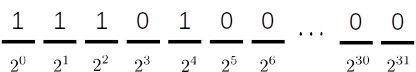
\includegraphics[width=0.75\columnwidth]{binary_23.png}
\caption{The number 23 in unsigned integer format.}
\label{fig:lec1n-binary-23}
\end{figure}


%\vspace{0.25cm}
%\noindent (image of 24 in binary)
%\vspace{0.25cm}

With 32-bit unsigned integers the computer can exactly represent all integers between 0 and $2^{32}-1$. Negative integers and integers greater than $2^{31}$ are not represented at all.%\sidenote{\textbf{Question:} What do you get from the following MATLAB code?
%\begin{lstlisting}[style=myMatlab]
%a = uint32(2^32-1);
%b = uint32(1);
%c = a + b;
%fprintf('c = %d \n',c);
%\end{lstlisting}

%\lstinline[style=myMatlab]{ a = uint32(2^32 - 1)  b = unit32(1) }

%\vspace{0.1cm}

%\noindent\textbf{Answer:} The variable c will still be equal to $2^{31}-1$.  MATLAB will round numbers outside of the range of representation for 32-bit unsigned ints to the nearest endpoint which, in this case, is $2^{31}-1$.
%}

\newthought{There are fewer} applications for which \emph{signed integers} will be used for this course, but they are, naturally, important.  Perhaps the most obvious way that a computer might represent signed integers would be to just use the same format as unsigned integers except to reserve one bit for the sign.  This is not, however, the way it is normally done.  For one thing, this approach results in there being two different bit-patterns for zero.  This is slightly inconvenient but not the sort of thing that passes without notice in computer engineering circles. Another, perhaps more significant, issue with this approach is that special logic would be needed when adding or subtracting a mixture of positive and negative integers. (i.e. you would not be able to use the same circuitry on the microprocessor for adding positive and negative numbers together as you would for two adding two positive numbers.)
  
The format that is normally used today for representing signed integers is called \emph{two's complement}.  If you want to write a positive number in two's complement format, you do the same thing as you would normally do for an unsigned integer.\sidenote[][-1.5cm]{Except, as it turns out, the largest positive 32-bit signed integer will only half as large as the corresponding largest signed integer.} If you need to write a negative number, you start by expressing the positive number, then you \emph{take the complement of each binary digit} and, when you are done with that, you \emph{add one.} A demonstration of this number representation, shortened to 5-bits to make it more compact, is shown in Figure \ref{fig:twos-complement-demo}.  


\begin{marginfigure}
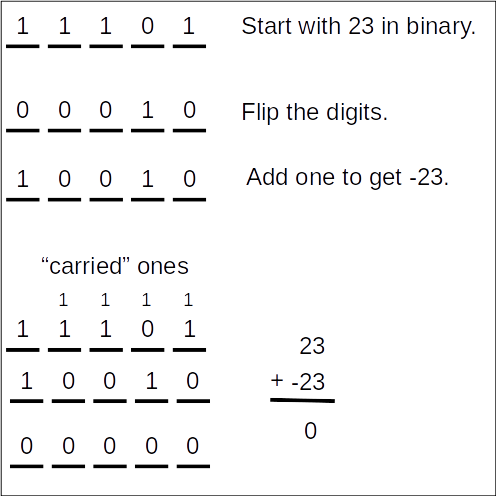
\includegraphics{twos-complement-demo.png}
\caption{Demonstration of twos-complement: adding 23 and -23 in 5-bit representation.}
\label{fig:twos-complement-demo}
\end{marginfigure}

%\vspace{0.25cm}
%\noindent (image showing example two's complement)
%\vspace{0.25cm}

This representation has the advantages that: a) there is only a single representation for zero; and b) the same hardware is used for both addition and subtraction (i.e. to subtract you simply add a negative number.)

\subsection{Floating Point Numbers}
In general, binary floating point numbers are given in the form shown in Equation \ref{eq:bfpn-format}:
\begin{equation}
1.\underbrace{\text{fff}\dots\text{f}}_{\text{mantissa}} \times 2^{\underbrace{\text{eee}\dots\text{e}}_{\text{exponent}}}
\label{eq:bfpn-format}
\end{equation}
where a number of digits available are divided between the fraction, or \emph{mantissa}, and \emph{exponent}.  In any finite machine, there will be a limit to the number of total digits available.  Thus an engineering decision needs to be made to determine how many digits will be allocated to the mantissa and how many for the exponent.  If you have more digits in the mantissa, you will be able to represent numbers that are closer together---the \emph{precision} of your representation will increase.  If you allocate more digits to the exponent, you will be able to represent numbers that are larger (for large positive exponents) or smaller (large negative exponents)---the \emph{range} of your representation will be wider.  The implications of these decisions should be clear: if you devote fewer bits to the mantissa, there will be more rounding errors in your calculations as real numbers are mapped, in some way, to the best floating point representation; if you devote fewer bits to the exponent, really large numbers and really small numbers will not be represented at all.  In earlier days of computing, different computer vendors made different decisions as to how floating point numbers would be represented.\cite{moler_fp1}  This caused problems when scientists tried to run the same code on different computers and got different results.  In 1985, the IEEE-754 standard was approved and, since then, has been adopted by essentially all computer manufacturers.  As a result, the menagerie of floating point formats and implementations have been tamed. Scientists and engineers could run their codes on different machines and expect to get the same results.

\begin{figure}
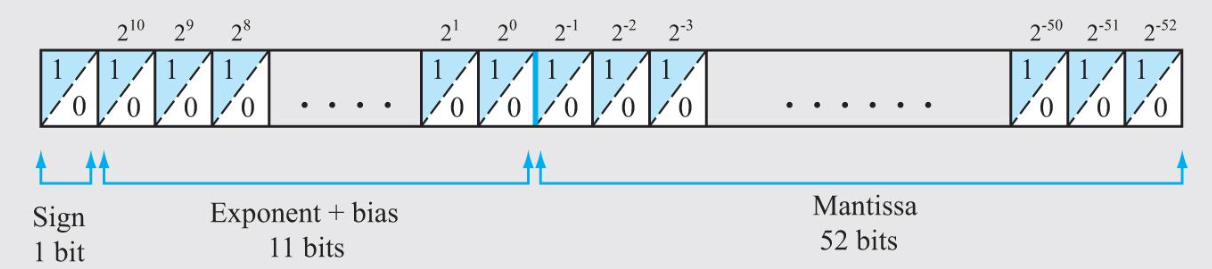
\includegraphics[width=0.94\columnwidth]{double-precision-format.png}
\caption{IEEE-754 double precision number format.}
\label{fig:double-precision-format}
\end{figure}

The IEEE-754 standard provides specification of several floating point number formats.  For this class, we will be concerned primarily with the \emph{double precision} floating point format which is illustrated in Figure \ref{fig:double-precision-format}.  This format uses a single sign bit (1 for negative, 0 for positive), 11 bits for the exponent which is encoded as an unsigned integer with bias,\sidenote{For double precision numbers, the bias is 1023.} and 52 bits for the mantissa.\sidenote{\textbf{Note:} The number 1 shown in Equation \ref{eq:bfpn-format} is not stored but is implicitly included in all \emph{normalized} floating point numbers.  This is done so that all numbers will have a \emph{unique} floating point representation. }  In the double precision format, the smallest positive number that can be represented is $2^{-1022}$ which is approximately equal to $2.2 \times 10^{-308}$.\marginnote{MATLAB includes built-in functions to report the smallest and largest representable floating point numbers.  The functions \lstinline[style=myMatlab]{realmin(precision)} and \lstinline[style=myMatlab]{realmax(precision)} will return the  smallest or largest positive floating point number for ``single'' or ``double'' precision floating point precision.} The smallest interval between numbers that can be represented is called \emph{machine epsilon}.\marginnote{In MATLAB, machine epsilon is provided with the function: \lstinline[style=myMatlab]{eps(precision)} for ``single'' and ``double'' precision.}  The size of this limit is driven by the number of bits in the mantissa.  For IEEE-754 double precision floating point numbers this is approximately $2.22 \times 10^{-16}$.\sidenote{Sometimes computational scientists refer to this as ``16 digits of precision.''}

\newthought{The procedure to} encode real numbers in the double precision floating point format will be illustrated with an example.

\vspace{0.5cm}

\noindent\textbf{Example:} Write the number -10.5 using the IEEE-754 double precision format.

\vspace{0.25cm}

\noindent\textbf{Step \#1:} Determine the mantissa and the exponent.  To do this, we normalize the number by dividing by $2^e$ where $e$ is the largest power of 2 that is \emph{less} than the magnitude of the number you are encoding.  

\vspace{0.1cm} 

\noindent In this case, $e=3$ since 10.5 is greater than $2^3$ but less than $2^4$.  

\begin{align*}
\frac{-10.5}{2^3} & = -1.3125 \\
\Rightarrow -10.5 &= -1.3125 \times 2^3
\end{align*}

\noindent Therefore the mantissa will need to encode 0.3215, and the exponent will need to encode 3 plus the bias of 1023, or 1026.

\vspace{0.25cm}

\noindent\textbf{Step \#2:} Set the sign bit. As the number is negative, the sign bit is: 1.

\vspace{0.25cm}


\noindent\textbf{Step \#3:} Calculate the 11 exponent bits.  

\begin{align*}
1026 &= 1024 + 2 \\
&= 1 \times 2^{10} + 1 \times 2^{1}
\end{align*}


\begin{figure}
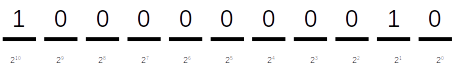
\includegraphics[width=0.75\columnwidth]{lec1n-ex1-exponent.png}
\caption{Exponent: 3+1023 = 1026 in 11-bit binary.}
\label{fig:lec1n-ex1-exponent}
\end{figure}   
  

\vspace{0.25cm}

\noindent\textbf{Step \#4:} Calculate the 52 mantissa bits to represent 0.3125.  The result is shown in Figure \ref{fig:lec1n-ex1-mantissa}.

\begin{figure}
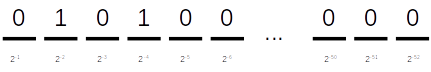
\includegraphics[width=0.75\columnwidth]{lec1n-ex1-mantissa.png}
\caption{Mantissa: 0.25 + 0.0625 = 0.3125.}
\label{fig:lec1n-ex1-mantissa}
\end{figure}

\noindent Where the calculations might be done as shown below:
\begin{align*}
0.3125 - 0 \times 2^{-1} &= 0.3125 \\
0.3125 - 1 \times 2^{-2} &= 0.0625 \\
0.0625 - 0 \times 2^{-3} &= 0.0625 \\
0.0625 - 1 \times 2^{-4} &= 0
\end{align*}
and all other entries are, of course, zero.


\section{Sources of Error} \index{error, truncation} \index{error, round-off} \index{error, modeling}

When using numerical methods there are several sources of error that you, as an engineer, should be aware of.  We have just discussed the details of double precision numbers so \emph{round-off error} is at the top of our mind.  Real numbers are not represented exactly on a computer but instead as floating point numbers.  The floating point number \emph{closest} to the real number gets used in its place. Error due to this round-off accumulates with mathematical operations.  Quantitative analysis of the accumulation of round-off-error is a tedious (albeit important) business that we will avoid in this class.  Nonetheless, engineers need to be aware that it is happening and, in a few instances, we will take steps to mitigate this build-up of error.

The second source of error that we will mention here is something that should be familiar to students who have taken the course in analytical methods: \emph{truncation error}.  In the analytical methods course we suffered from truncation error every time we shortened our infinite series solution to a finite number of terms.  We reduced this error by increasing the number of terms we retained, but there was no way to make it go away completely.  In this course we will see further instances of truncation error in most every algorithm we implement.  Derivatives and integrals that could, in principle, be done exactly, will be done approximately as we truncate the Taylor series expansion or limit the order of polynomials used to represent the exact derivative or integral.  We can reduce the magnitude of these errors, but we cannot make them go away entirely.

The third source of error mentioned here is \emph{modeling error}.  Modeling errors are reflected in the differences between observed physical phenomena and the corresponding mathematical model of the phenomena.  There are a couple of reasons for these differences and these include:
\begin{enumerate}
\item Linearization of non-linear processes.  Instances where you may already have done this, in your heat transfer or fluid dynamics class, include:
\begin{enumerate}
\item Assumption of constant thermal conductivity for heat conduction problems.  This assumption linearizes the heat equation and, for simple geometry, renders the problem amenable to analytical methods.  This assumption is retained for many numerical methods when solving the heat equation on more complex geometry.  The modeling error resulting from linearization remains.

\item Assumption of constant drag coefficient for external flow calculations.  Once again, this assumption simplifies the calculations at the cost of model fidelity.
\end{enumerate}

\item De-coupling of physical processes.  Nature does not specialize its behavior by academic subjects.  Consequently the air flowing over the control surfaces of a fighter jet is both a fluid dynamics and structural dynamics problem when the wing responds to forces imposed by the air.  Water flowing through a pressurized water reactor core is heated by forced convection and radiation that you might calculate in heat transfer class, but the resulting change in water properties also affect the neutron economy and power production rate that you might calculate in reactor physics which, in turn, will have further effect on the heat transfer problem.  We de-couple these processes so the analysis is more manageable but as a result the solution we arrive at is in error.  

\end{enumerate}  
Scientists and engineers need to be aware of all of these sources of errors and take steps to mitigate them where possible.



